\documentclass[hyperref={pdfpagelabels=false},svgnames]{beamer}
\mode<presentation>{
  \usetheme{Madrid}
  \setbeamertemplate{navigation symbols}{}
}
\usepackage[english]{babel}
\usepackage[latin1]{inputenc}
\usepackage{times}
\usepackage[T1]{fontenc}
\usepackage{graphicx}
\usepackage{tikz}
\usepackage{listings}

\lstset{%
language=C,
basicstyle=\footnotesize,
}

\title{Operating systems and concurrency B04}
\subtitle{}
\author{David Kendall}
\institute{Northumbria University}
\date{}

\begin{document}

\begin{frame}
\titlepage
\end{frame}

\begin{frame}
\frametitle{Introduction}
\begin{itemize}
\item Towards an operating system: CMSIS and Mbed
\item Multi-tasking operating system services
\item $\mu$C/OS-II (uC/OS-II) 
\item Task management in uC/OS-II
\end{itemize}
\end{frame}

\begin{frame}[shrink=10, fragile]
\frametitle{Standard names for the microcontroller registers}
\begin{columns}
\column{.6\textwidth}
\begin{lstlisting}
#include <stdbool.h>
#include <stdint.h>
#include <LPC407x_8x_177x_8x.h>

#define LED1PIN    (1UL << 18)

void delay(uint32_t ms);

int main() {
  LPC_IOCON->P1_18 &= ~0x1FUL;
  LPC_GPIO1->DIR |= LED1PIN;
  while (true) {
    LPC_GPIO1->SET = LED1PIN;
    delay(1000);
    LPC_GPIO1->CLR = LED1PIN;
    delay(1000);
  }
}
\end{lstlisting}
\column{.4\textwidth}
\begin{itemize}
\item Header file \verb'LPC407x_8x_177x_8x.h' provided by the 
manufacturer of the microcontroller (NXP) to give a set of
\alert{standard names} for the microcontroller registers
\item No need to write \verb'#define's after looking up the
addresses yourself.
\item Header file written in standard ANSI C - CMSIS-complaint -
  portable between tool providers.
\end{itemize}
\end{columns}
\end{frame}
 
\begin{frame}[fragile]
\frametitle{CMSIS}
\begin{columns}
\column{.5\textwidth}
\begin{itemize}
\item Cortex Microcontroller Software Interface Standard
\item CMSIS-Core
\begin{itemize}
\item Standard set of names provided by ARM for accessing
the microprocessor
\item Standard startup files for bringing up the CPU out of reset:
\begin{itemize}
\item configure system clocks
\item define the vector table
\item run the \verb'main' function
\end{itemize}
\end{itemize}
\item Improves software portability and reusability across
different microcontrollers and toolchains
\end{itemize}
\column{.5\textwidth}
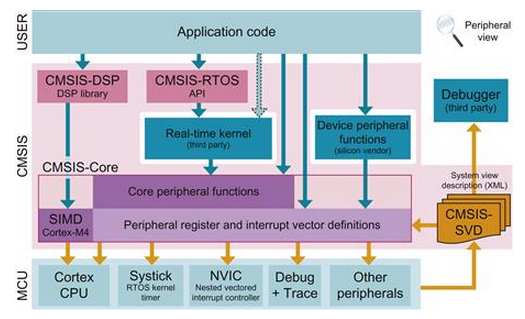
\includegraphics[width=\textwidth]{cmsis}
\par
\begin{tiny}
Martin, T. \emph{The Designer's Guide to the Cortex-M Processor Family: A Tutorial Approach}, Newnes, 2013
\end{tiny}
\end{columns}
\end{frame}


\begin{frame}
\frametitle{Foreground/background tasks}
\begin{columns}[c]
\column{.4\textwidth}
\begin{itemize}
\item Simple multitasking
\item Super loop calls functions
for computation (background)
\item Interrupt service routines (ISRs) handle
asynchronous events (foreground)
\end{itemize}
\column{.5\textwidth}
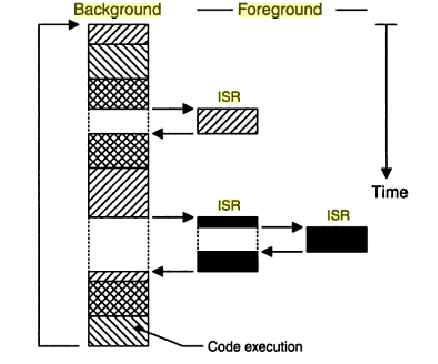
\includegraphics[width=\textwidth]{fig1}
\end{columns}
\uncover<2->{%
\begin{block}{Problem}
Model with only one computation task is not flexible enough
\end{block}}
\end{frame}

\begin{frame}
\frametitle{Multitasking}
\begin{itemize}
\item Easier to structure the application as a set of 
\alert{concurrent} tasks rather than as a single program or as
foreground/background tasks: each task is responsible for
some well-defined part of the system's overall behaviour
\item But only the illusion of concurrency - the OS
switches quickly between tasks, executing some instructions
from one task before moving on to another task
\item switching from one text to another requires a
\alert{context switch}
\item deciding which task to switch to requires a 
\alert{scheduling algorithm}
\end{itemize}
\end{frame}


\begin{frame}
\frametitle{Scheduling}
\begin{itemize}
\item Deciding when one task should stop executing and
which one should begin next is a \alert{scheduling} problem
\item Two main approaches to scheduling:
\begin{itemize}
\item Preemptive scheduling
\begin{itemize}
\item Task is \alert{forced to yield} the CPU
\item Round robin
\item Priority-based
\end{itemize}
\item Non-preemptive (cooperative) scheduling
\begin{itemize}
\item Task \alert{voluntarily yields} the CPU and signals
the next task to begin
\end{itemize}
\end{itemize}
\end{itemize}
\end{frame}


\begin{frame}
\frametitle{Fixed-priority preemptive scheduling}
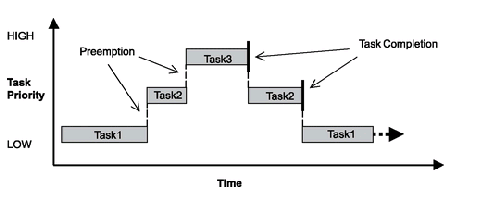
\includegraphics[width=.9\textwidth]{fig5}
\begin{itemize}
\item We focus on fixed-priority premptive scheduling
\end{itemize}
\end{frame}

\begin{frame}
\frametitle{A task and its execution states}
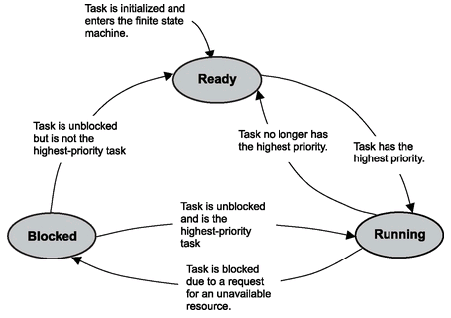
\includegraphics[width=.9\textwidth]{fig3}
\end{frame}


\begin{frame}
\frametitle{uC/OS-II: A small operating system}
\begin{itemize}
\item Main features:
\begin{itemize}
\item Multi-tasking
\item Preemptive
\end{itemize}
\item Other features:
\begin{itemize}
\item Predictable
\item Robust and reliable
\item Standards-compliant
\item Portable
\item Scalable
\item Source code available
\end{itemize}
\end{itemize}
\end{frame}

\begin{frame}
\frametitle{uC/OS-II Services}
\begin{itemize}
\item<1-> Task management
\item<1-> Delay management
\item<2-> Semaphores
\item<2-> Mutual exclusion semaphores
\item<2-> Event flags
\item<2-> Message mailboxes
\item<2-> Message queues
\item<2-> Memory management
\item<2-> Timers
\item<2-> Miscellaneous
\end{itemize}

\uncover<3->{%
See \href{http://cgweb1.northumbria.ac.uk/SubjectAreaResources/embedded/micrium/QuickRefChart-Color.pdf}{\textcolor{blue}{uC/OS-II Quick Reference}}}
\end{frame}

\begin{frame}[fragile]
\frametitle{Tasks behaviour}
\begin{itemize}
\item The behaviour of a task is defined by a C function that:
\begin{enumerate}
\item never terminates
\item blocks repeatedly
\end{enumerate}
\end{itemize}

\begin{block}{Example of task behaviour definition}

\begin{lstlisting}
static void appTaskLED2(void *pdata) {
  while (true) {                
    OSTimeDlyHMSM(0,0,0,500);   
    gpioPinToggle(&pin[LED2]);
  } 
}
\end{lstlisting}

\end{block}
\end{frame}


\begin{frame}[fragile]
\frametitle{Tasks: other requirements}
\begin{block}{Priority}
\begin{itemize}
\item Used for fixed-\alert{priority} pre-emptive scheduling
\item a number between 0 and \verb'OS_LOWEST_PRIO'
\item \alert{low} number $\Rightarrow$ \alert{high} priority
\item \alert{high} number $\Rightarrow$ \alert{low} priority
\item OS reserves priorities 0 to 3 and \verb'OS_LOWEST_PRIO' - 3 to \verb'OS_LOWEST_PRIO'
\item Advice: define an enumeration of task priority constants, starting at
priority level 4.
\item Example
\begin{lstlisting}
enum {
  APP_TASK_BUTTONS_PRIO = 4,
  APP_TASK_LED1_PRIO,
  APP_TASK_LED2_PRIO
};
\end{lstlisting}
\end{itemize}
\end{block}
\end{frame}


\begin{frame}[fragile]
\frametitle{Tasks: other requirements}
\begin{block}{Stack}
\begin{itemize}
\item Each task needs its own data area (\alert{stack}) for storing
\begin{itemize}
\item context
\item local variables
\end{itemize}
\item Example stack definition

\begin{lstlisting}
enum {APP_TASK_LED2_STK_SIZE = 256};
static OS_STK appTaskLED2Stk[APP_TASK_LED2_STK_SIZE];
\end{lstlisting}

\end{itemize}
\end{block}

\pause

\begin{block}{User data}
\begin{itemize}
\item Optionally tasks can be given access to user data when
they are created
\item We will not use this feature in this module
\item Advice: always specify this as \verb'(void *)0' when
creating a task
\end{itemize}
\end{block}
\end{frame}


\begin{frame}[fragile]
\frametitle{Task creation}
\lstset{basicstyle=\scriptsize, frame=single}
\begin{itemize}
\item A task is created using the OS function 

\begin{lstlisting}
INT8U OSTaskCreate(
        void (*task)(void *pdata), /* function for the task   */
        void *pdata,               /* user data for function  */
        OS_STK *ptos,              /* pointer to top of stack */
        INT8U priority             /* task priority           */
);
\end{lstlisting}

\end{itemize}

\pause

\begin{block}{Example}
\begin{lstlisting}
enum {APP_TASK_LED2_PRIO = 4};
enum {APP_TASK_LED2_STK_SIZE = 256};

static OS_STK appTaskLED2Stk[APP_TASK_LED2_STK_SIZE];

OSTaskCreate(appTaskLED2,                               
             (void *)0,
             (OS_STK *)&appTaskLED2Stk[APP_TASK_LED2_STK_SIZE - 1],
             APP_TASK_LED2_PRIO);
\end{lstlisting}

\end{block}
\end{frame}


\begin{frame}[fragile]
\frametitle{Task delay}
\begin{itemize}
\item Often, a task will block itself by explicitly asking the OS to delay it
for some period of time
\item \verb'void OSTimeDly(INT16U ticks);'
\item Causes a context switch if \verb'ticks' is between 1 and 65535
\item If \verb'ticks' is 0, \verb'OSTimeDly()' returns immediately to
  caller
\item On context switch uC/OS-II executes the next highest priority task
\item Task that called \verb'OSTimeDly()' will be made ready to run when
  the specified number of ticks elapses - actually runs when it becomes the
  highest priority ready task
\item Resolution of the delay is between 0 and 1 tick
\item Another task can cancel the delay by calling \verb'OSTimeDlyResume()'
\end{itemize}
\end{frame}


\begin{frame}[fragile]
\frametitle{Task delay}
\begin{itemize}
\item \verb'OSTimeDly()' specifies delay in terms of a number of ticks
\item Use \verb'OSTimeDlyHMSM()' to specify delay in terms of \alert{H}ours,
 \alert{M}inutes, \alert{S}econds and \alert{M}illiseconds
\item Otherwise \verb'OSTimeDlyHMSM()' behaves as \verb'OSTimeDly()'
\end{itemize}
\end{frame}

\lstset{basicstyle=\tiny}


\begin{frame}[fragile]
\frametitle{Complete example}

\begin{lstlisting}
#include <stdbool.h>
#include <ucos_ii.h>
#include "gpioPin.h"

typedef enum {
  APP_TASK_LED1_PRIO = 4,
  APP_TASK_LED2_PRIO
} taskPriorities_t;

typedef enum {
  APP_TASK_LED1_STK_SIZE = 256,
  APP_TASK_LED2_STK_SIZE = 256
} stackSizes_t;

static OS_STK appTaskLED1Stk[APP_TASK_LED1_STK_SIZE];
static OS_STK appTaskLED2Stk[APP_TASK_LED2_STK_SIZE];

static void appTaskLED1(void *pdata);
static void appTaskLED2(void *pdata);

typedef enum {
	LED1 = 0,
	LED2
} deviceNames_t;

gpioPin_t pin[2];

\end{lstlisting}

\end{frame}

\begin{frame}[fragile]
\frametitle{Complete example}

\begin{lstlisting}
int main() {

  /* Initialise the GPIO pins */
  gpioPinInit(&pin[LED1], 1, 18, OUTPUT_PIN);
  gpioPinInit(&pin[LED2], 0, 13, OUTPUT_PIN);

  /* Initialise the OS */
  OSInit();                                                  

  /* Create the tasks */
  OSTaskCreate(appTaskLED1,                              
               (void *)0,
               (OS_STK *)&appTaskLED1Stk[APP_TASK_LED1_STK_SIZE - 1],
               APP_TASK_LED1_PRIO);
 
  OSTaskCreate(appTaskLED2,                              
               (void *)0,
               (OS_STK *)&appTaskLED2Stk[APP_TASK_LED2_STK_SIZE - 1],
               APP_TASK_LED2_PRIO);

 
  /* Start the OS */
  OSStart();                                                 
 
  /* Should never arrive here */
  return 0;     
}
\end{lstlisting}
\end{frame}

\begin{frame}[fragile]
  \frametitle{Complete example}
  \begin{lstlisting}
static void appTaskLED1(void *pdata) {
  /* Start the OS ticker -- must be done in the highest priority task */
  SysTick_Config(SystemCoreClock / OS_TICKS_PER_SEC);
 
  /* Task main loop */
  while (true) {
    gpioPinToggle(&pin[LED1]);
    OSTimeDlyHMSM(0,0,0,500);
  }
}

static void appTaskLED2(void *pdata) {
  while (true) {
    gpioPinToggle(&pin[LED2]);
    OSTimeDlyHMSM(0,0,0,500);
  }
}
\end{lstlisting}

\end{frame}


\begin{frame}
\frametitle{Acknowledgements}
\begin{itemize}
\item Qing Li and Caroline Yao, Real-time concepts for embedded systems, CMP, 2003
\item Jean Labrosse, MicroC/OS-II: The Real-Time Kernel, CMP, 2002
\end{itemize}
\end{frame}

\end{document}


